%----------------------------------------------------------------------------------------
%	PACKAGES AND OTHER DOCUMENT CONFIGURATIONS
%----------------------------------------------------------------------------------------

\documentclass[paper=a4, fontsize=11pt]{scrartcl} % A4 paper and 11pt font size

% ---- Entrada y salida de texto -----

\usepackage[T1]{fontenc} % Use 8-bit encoding that has 256 glyphs
\usepackage[utf8]{inputenc}
%\usepackage{fourier} % Use the Adobe Utopia font for the document - comment this line to return to the LaTeX default

% ---- Idioma --------

\usepackage[spanish, es-tabla]{babel} % Selecciona el español para palabras introducidas automáticamente, p.ej. "septiembre" en la fecha y especifica que se use la palabra Tabla en vez de Cuadro

% ---- Otros paquetes ----
\usepackage{csquotes} %Para permitir el uso de comillas Quotes https://tex.stackexchange.com/questions/36812/isnt-there-any-other-way-of-doing-double-quotes-in-latex-besides
\usepackage[hyphens]{url} % ,href} %para incluir URLs e hipervínculos dentro del texto (aunque hay que instalar href)
\usepackage{hyperref}
\usepackage{color}
\usepackage{graphics,graphicx, floatrow} %para incluir imágenes y notas en las imágenes
\usepackage{graphics,graphicx, float} %para incluir imágenes y colocarlas

\graphicspath {{./img/}}

\usepackage{listings}  %para introducir comandos

\lstdefinestyle{mybash}
{basicstyle=\ttfamily,
  showstringspaces=false,
  commentstyle=\color{red},
  keywordstyle=\color{blue},
  language=bash,
  alsoletter=/,
  basicstyle=\footnotesize,
  numbers=left,
  stepnumber=1,
  showstringspaces=false,
  tabsize=1,
  breaklines=true,
  breakatwhitespace=false,
}
\lstdefinestyle{mysql}
{basicstyle=\ttfamily,
  showstringspaces=false,
  commentstyle=\color{red},
  keywordstyle=\color{blue},
  language=sql,
  basicstyle=\footnotesize,
  numbers=left,
  stepnumber=1,
  showstringspaces=false,
  tabsize=1,
  breaklines=true,
  breakatwhitespace=false,
}


% Para hacer tablas comlejas
%\usepackage{multirow}
%\usepackage{threeparttable}

%\usepackage{sectsty} % Allows customizing section commands
%\allsectionsfont{\centering \normalfont\scshape} % Make all sections centered, the default font and small caps

\usepackage{fancyhdr} % Custom headers and footers
\pagestyle{fancyplain} % Makes all pages in the document conform to the custom headers and footers
\fancyhead{} % No page header - if you want one, create it in the same way as the footers below
\fancyfoot[L]{} % Empty left footer
\fancyfoot[C]{} % Empty center footer
\fancyfoot[R]{\thepage} % Page numbering for right footer
\renewcommand{\headrulewidth}{0pt} % Remove header underlines
\renewcommand{\footrulewidth}{0pt} % Remove footer underlines
\setlength{\headheight}{13.6pt} % Customize the height of the header

\setlength\parindent{0pt} % Removes all indentation from paragraphs - comment this line for an assignment with lots of text

\newcommand{\horrule}[1]{\rule{\linewidth}{#1}} % Create horizontal rule command with 1 argument of height


%----------------------------------------------------------------------------------------
%	TÍTULO Y DATOS DEL ALUMNO
%----------------------------------------------------------------------------------------
\graphicspath{ {img/} }

\title{
\normalfont \normalsize

\includegraphics[width=6cm,height=6cm]{logo}\\
\textsc{\textbf{Bootcamp Especialidad GNU/Linux (2023)}} \\ [25pt] % Your university, school and/or department name(s)
\horrule{0.5pt} \\[0.4cm] % Thin top horizontal rule
\huge Lab 04 - Procesos, servicios, demonios y su monitorización \\ % The assignment title
\horrule{2pt} \\[0.5cm] % Thick bottom horizontal rule
}


%https://es.overleaf.com/learn/latex/Inserting_Images
%Ruta relativa de   imagenes

\author{Pedro Antonio Mayorgas Parejo} % Nombre y apellidos

\date{\normalsize\today} % Incluye la fecha actual

%----------------------------------------------------------------------------------------
% DOCUMENTO
%----------------------------------------------------------------------------------------

\begin{document}

\maketitle % Muestra el Título

\newpage %inserta un salto de página

\tableofcontents % para generar el índice de contenidos

\newpage

%----------------------------------------------------------------------------------------
%	Cuestión 1
%----------------------------------------------------------------------------------------

\section{Usuario remoto y configuración de SSHD}

Creamos un usuario remoto que permita el acceso con SSH, para ello tenemos que tener un usuario que podamos autenticar  en el servidor.

\begin{lstlisting}[style=mybash]
# Creamos el usuario
sudo adduser pedrolab04
# Editamos el fichero de sshd
sudo nano /etc/ssh/sshd_config
\end{lstlisting}

Las configuraciones editadas son las siguientes:

\begin{figure}[H]
	\centering
	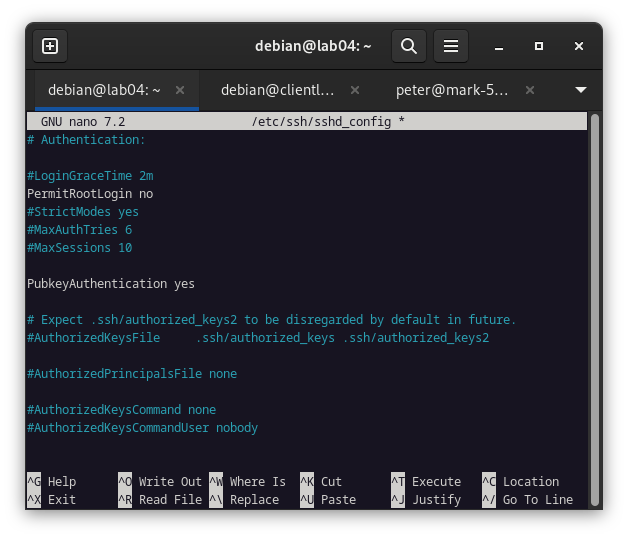
\includegraphics[scale=0.40]{00}
	\caption{Aquí indicamos las opciones de seguridad de no autenticar el usuario root y permitir por norma general la autenticación por clave pública.}
\end{figure}

\begin{figure}[H]
	\centering
	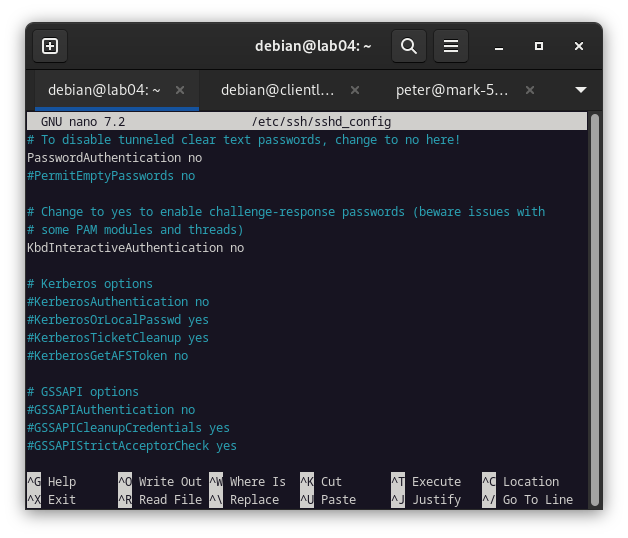
\includegraphics[scale=0.40]{01}
	\caption{Aquí desactivamos la autenticación por contraseña por norma general, forzando el uso de par de claves.}
\end{figure}

\begin{figure}[H]
	\centering
	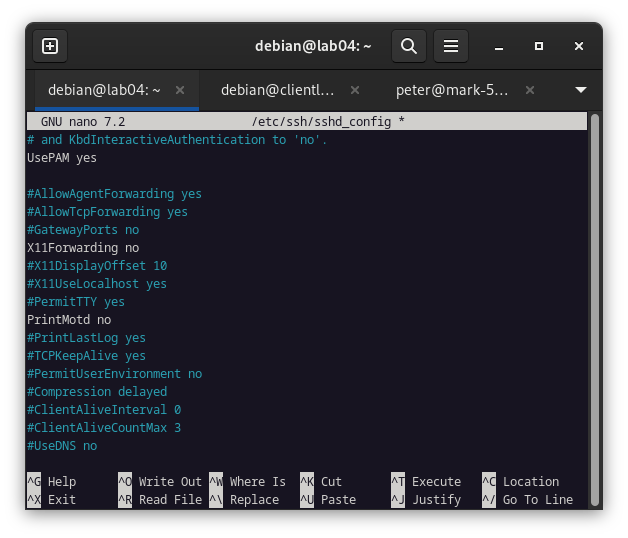
\includegraphics[scale=0.40]{02}
	\caption{Aquí desactivamos el uso de X11 ya que el servidor no tiene entorno gráfico.}
\end{figure}

\begin{figure}[H]
	\centering
	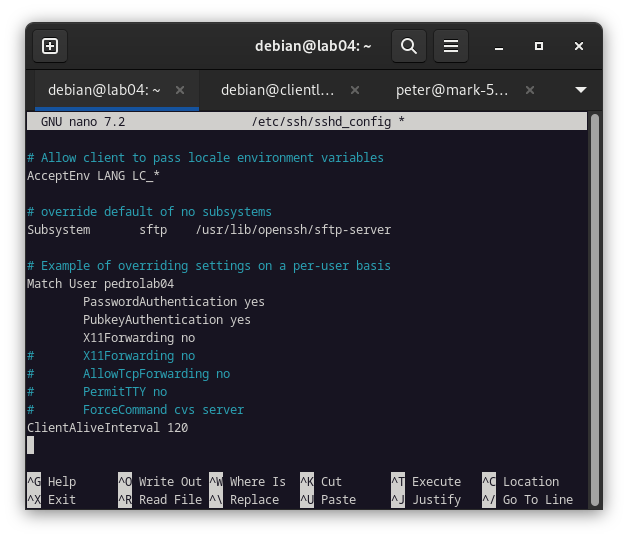
\includegraphics[scale=0.40]{03}
	\caption{Aquí hacemos un mach del usuario que se ha creado para la conectividad SSH, se permite el uso de contraseña para permitir la copia de la clave con ssh-copy-id.}
\end{figure}

\begin{figure}[H]
	\centering
	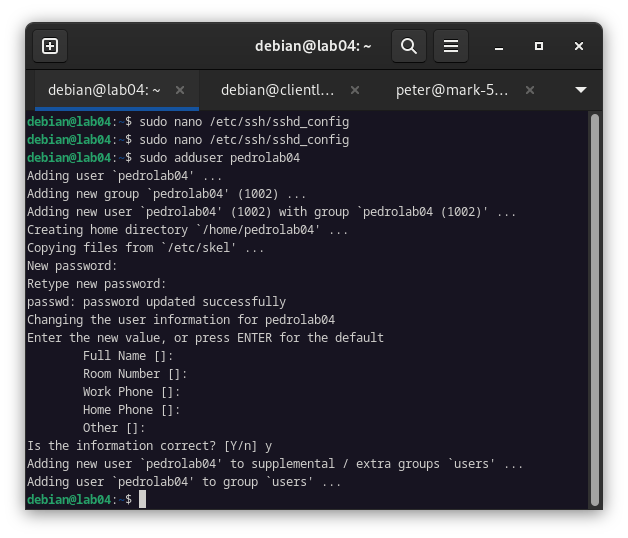
\includegraphics[scale=0.40]{04}
	\caption{Creación del usuario.}
\end{figure}

Ahora reiniciamos el servicio de sshd, para aplicar los cambios y verificamos que no exista ningún error de configuración.

\begin{figure}[H]
	\centering
	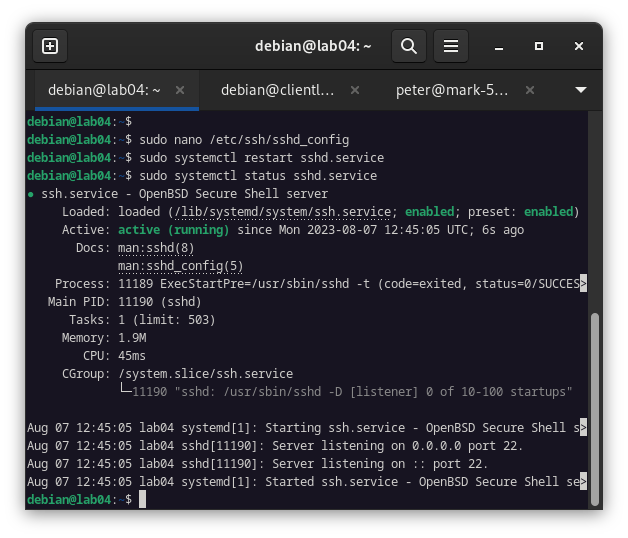
\includegraphics[scale=0.40]{05}
	\caption{Reinicio del servicio de SSHd.}
\end{figure}

\begin{lstlisting}[style=mybash]
sudo systemctl restart sshd.service
sudo systemctl status sshd.service
\end{lstlisting}

\newpage
\section{Proceso de generación de par de claves en el cliente y copia en el servidor}

Ahora en el cliente debemos crear un par de claves de RSA, para poder usarlas para autenticación sin contraseña en el lado del servidor. El comando utilizado es:

\begin{lstlisting}[style=mybash]
ssh-keygen
\end{lstlisting}

\begin{figure}[H]
	\centering
	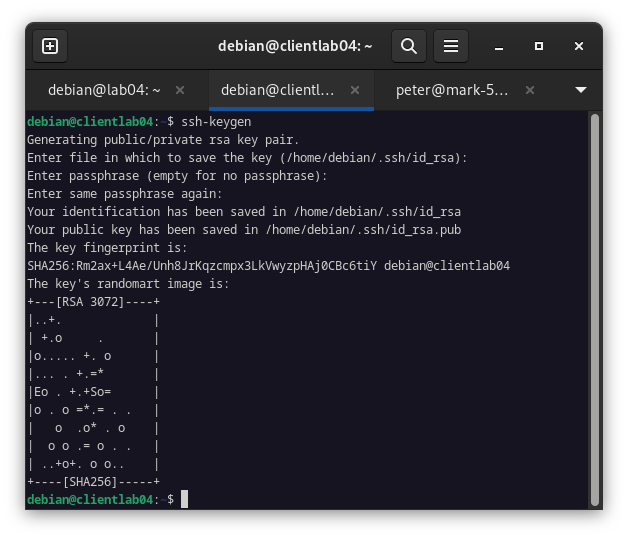
\includegraphics[scale=0.40]{06}
	\caption{Generación de la clave.}
\end{figure}

Una vez generada debemos copiarla en el servidor de destino hacia el usuario con el que queramos autenticarnos, en este caso pedrolab04, dicho usuario cuando se autentique copiará la clave pública id\_rsa.pub que se almacenará en su HOME, en concreto en un directorio oculto localizado en \textbf{.ssh/authorized\_keys}.
\vspace{5mm}

Comando para la copia de la clave:
\begin{lstlisting}[style=mybash]
ssh-copy-id pedrolab04@192.168.122.59
\end{lstlisting}

\begin{figure}[H]
	\centering
	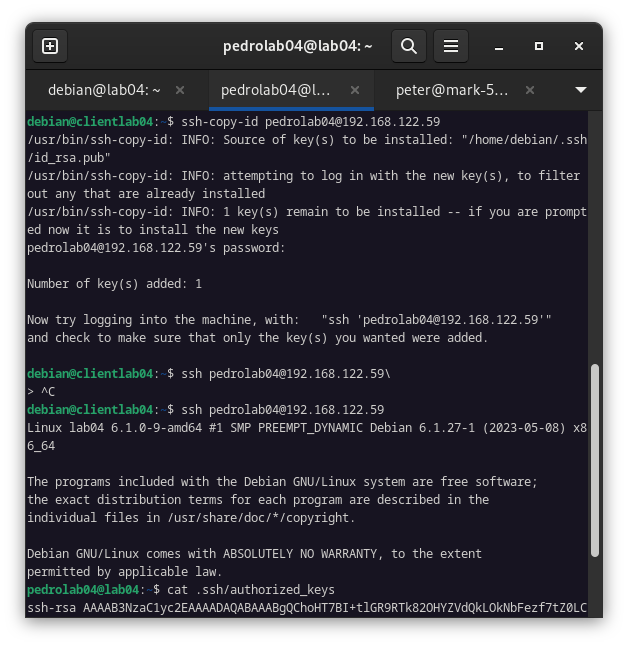
\includegraphics[scale=0.40]{07}
	\caption{Copia de la clave y autenticación sin contraseña.}
\end{figure}

\begin{figure}[H]
	\centering
	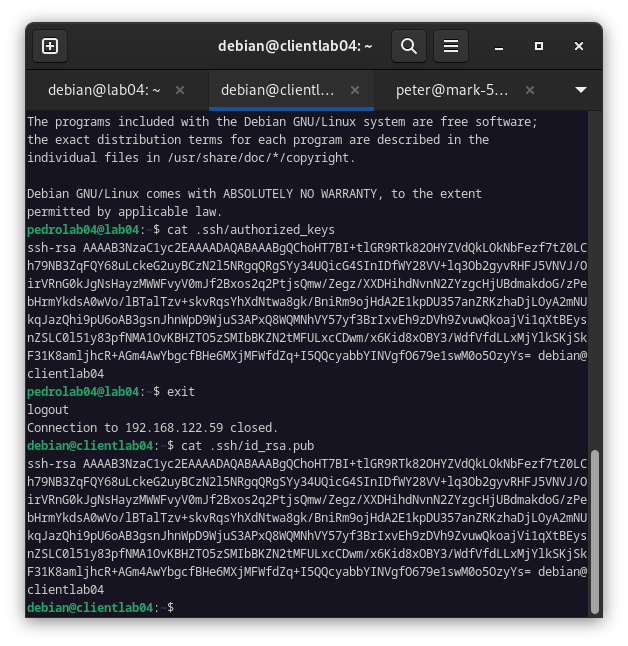
\includegraphics[scale=0.40]{08}
	\caption{Comparación del fichero authorized\_keys con la clave públicas.}
\end{figure}

Una vez termiando, debemos realizar el siguiente cambio para desactivar la autenticación por contraseña y permitir solo el uso de clave pública.

\begin{figure}[H]
	\centering
	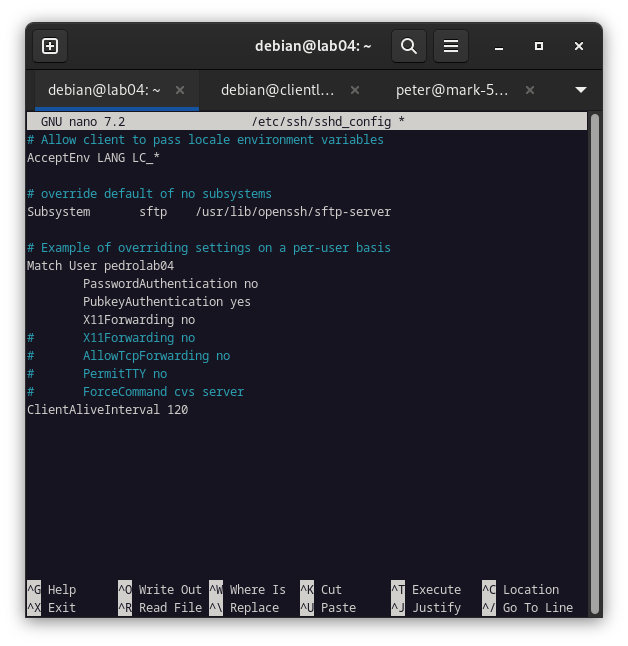
\includegraphics[scale=0.40]{09}
	\caption{Desactivación del uso de contraseñas.}
\end{figure}

Finalmente reiniciamos el servicio.

\begin{lstlisting}[style=mybash]
sudo systemctl restart sshd.service
sudo systemctl status sshd.service
\end{lstlisting}

\newpage
\section{Logs de ssh}

Antes en el intento de copiar la clave, he realizado un intento erróneo para poder generar entradas en el log de intentos fallados y de intentos legítimos. En primer lugar después de iniciar el servicio, se puede ver un intento fallido de pedrolab04 con contraseña incorrecta, luego se puede ver un intento legítimo que se corrresponde con el de la copia de la clave que es un comando generalmente y finalmente la autenticación sin contraseña legítima después de realizar la copia de seguridad.

El comando utilizado para ver dicho log es \textbf{journalctl}, en concreto con los siguientes parámetros:

\begin{lstlisting}[style=mybash]
sudo journalctl -u ssh
\end{lstlisting}

\begin{figure}[H]
	\centering
	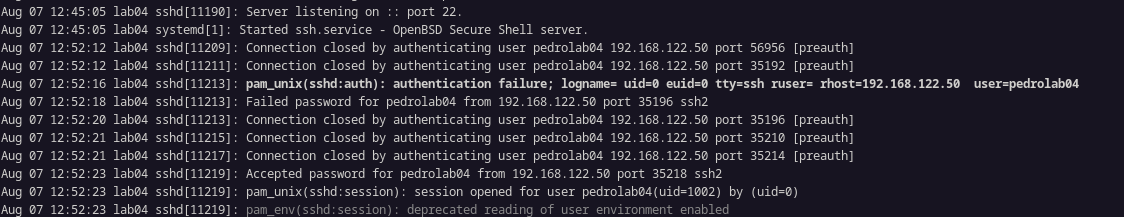
\includegraphics[scale=0.40]{10}
	\caption{Fallo de intento de contraseña y intento correcto con copia de clave visto en el log.}
\end{figure}

\begin{figure}[H]
	\centering
	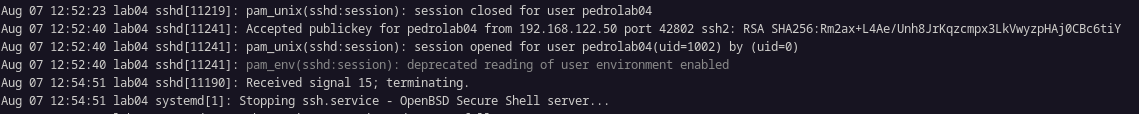
\includegraphics[scale=0.40]{11}
	\caption{Uso del par de claves visto en el log.}
\end{figure}

\begin{figure}[H]
	\centering
	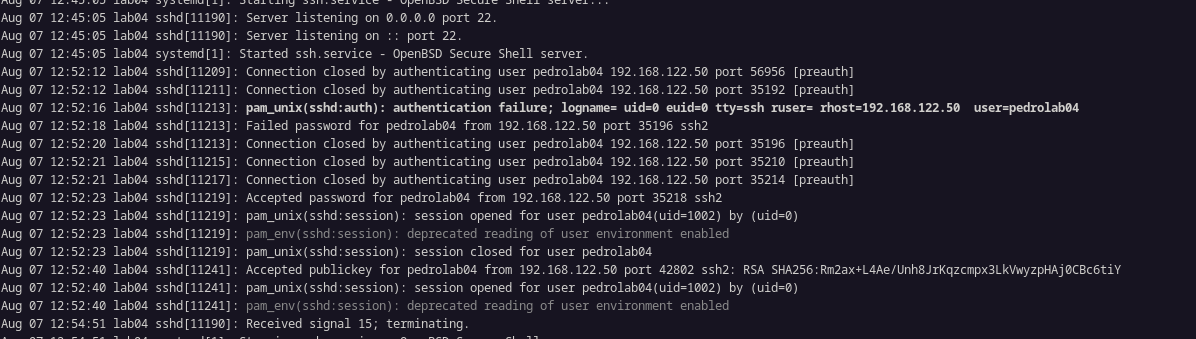
\includegraphics[scale=0.40]{12}
	\caption{Visión general de todo el proceso en el log.}
\end{figure}


Fuentes \footnote{\url{https://manpages.debian.org/testing/openssh-server/sshd\_config.5.en.html\#LogLevel}} \footnote{\url{https://manpages.debian.org/testing/openssh-client/ssh\_config.5.en.html}}

% \vspace{5mm}


% \begin{lstlisting}[style=mybash]
%     # Para una base de datos concreta
%     mysqldump --user=tiendabd --password=password --databases tiendabd --add-drop-database --add-drop-table [--replace] --host=127.0.0.1 --result-file=dump.sql
% \end{lstlisting}



%\begin{figure}[H]
%	\centering
%	\includegraphics[scale=0.40]{cuestion_1_1}
%	\caption{Se puede ver que al no haber un fallo grave, el sistema lo nota como que sigue funcionando pero en un estado degradado.}
%\end{figure}

%\newpage

%Se pueden hacer include en latex
%\newpage

\section{Section}

\subsection{Subseccion}

\subsubsection{Subseccion}



%-------Bibliografia-----------------------------

%\newpage
\section{Bibliografía}

% Ejemplo
\footnote{Administración de mdadm - Por Red Hat}
\textcolor{blue}{\url{https://access.redhat.com/documentation/en-us/red_hat_enterprise_linux/8/html/managing_storage_devices/managing-raid_managing-storage-devices#monitoring-raid_managing-raid}}



\end{document}
